\subsection{Forward Time-Of-Flight (FTOF)}

\subsubsection{Geometry}

The FTOF geometry is implemented through the java geometry service.
The service provides the Geant4 definitions that are read by the GEMC perl API to build the geometry database.

Each scintillator is a separate Geant4 volume. The paddles are assigned the scintillator material and
associated with the FTOF hit process routine.
Each scintillator is a box volume embedded in a trapezoidal mother volume made of air (see \F{ftofGeometry}).

\begin{figure}
	\centering
	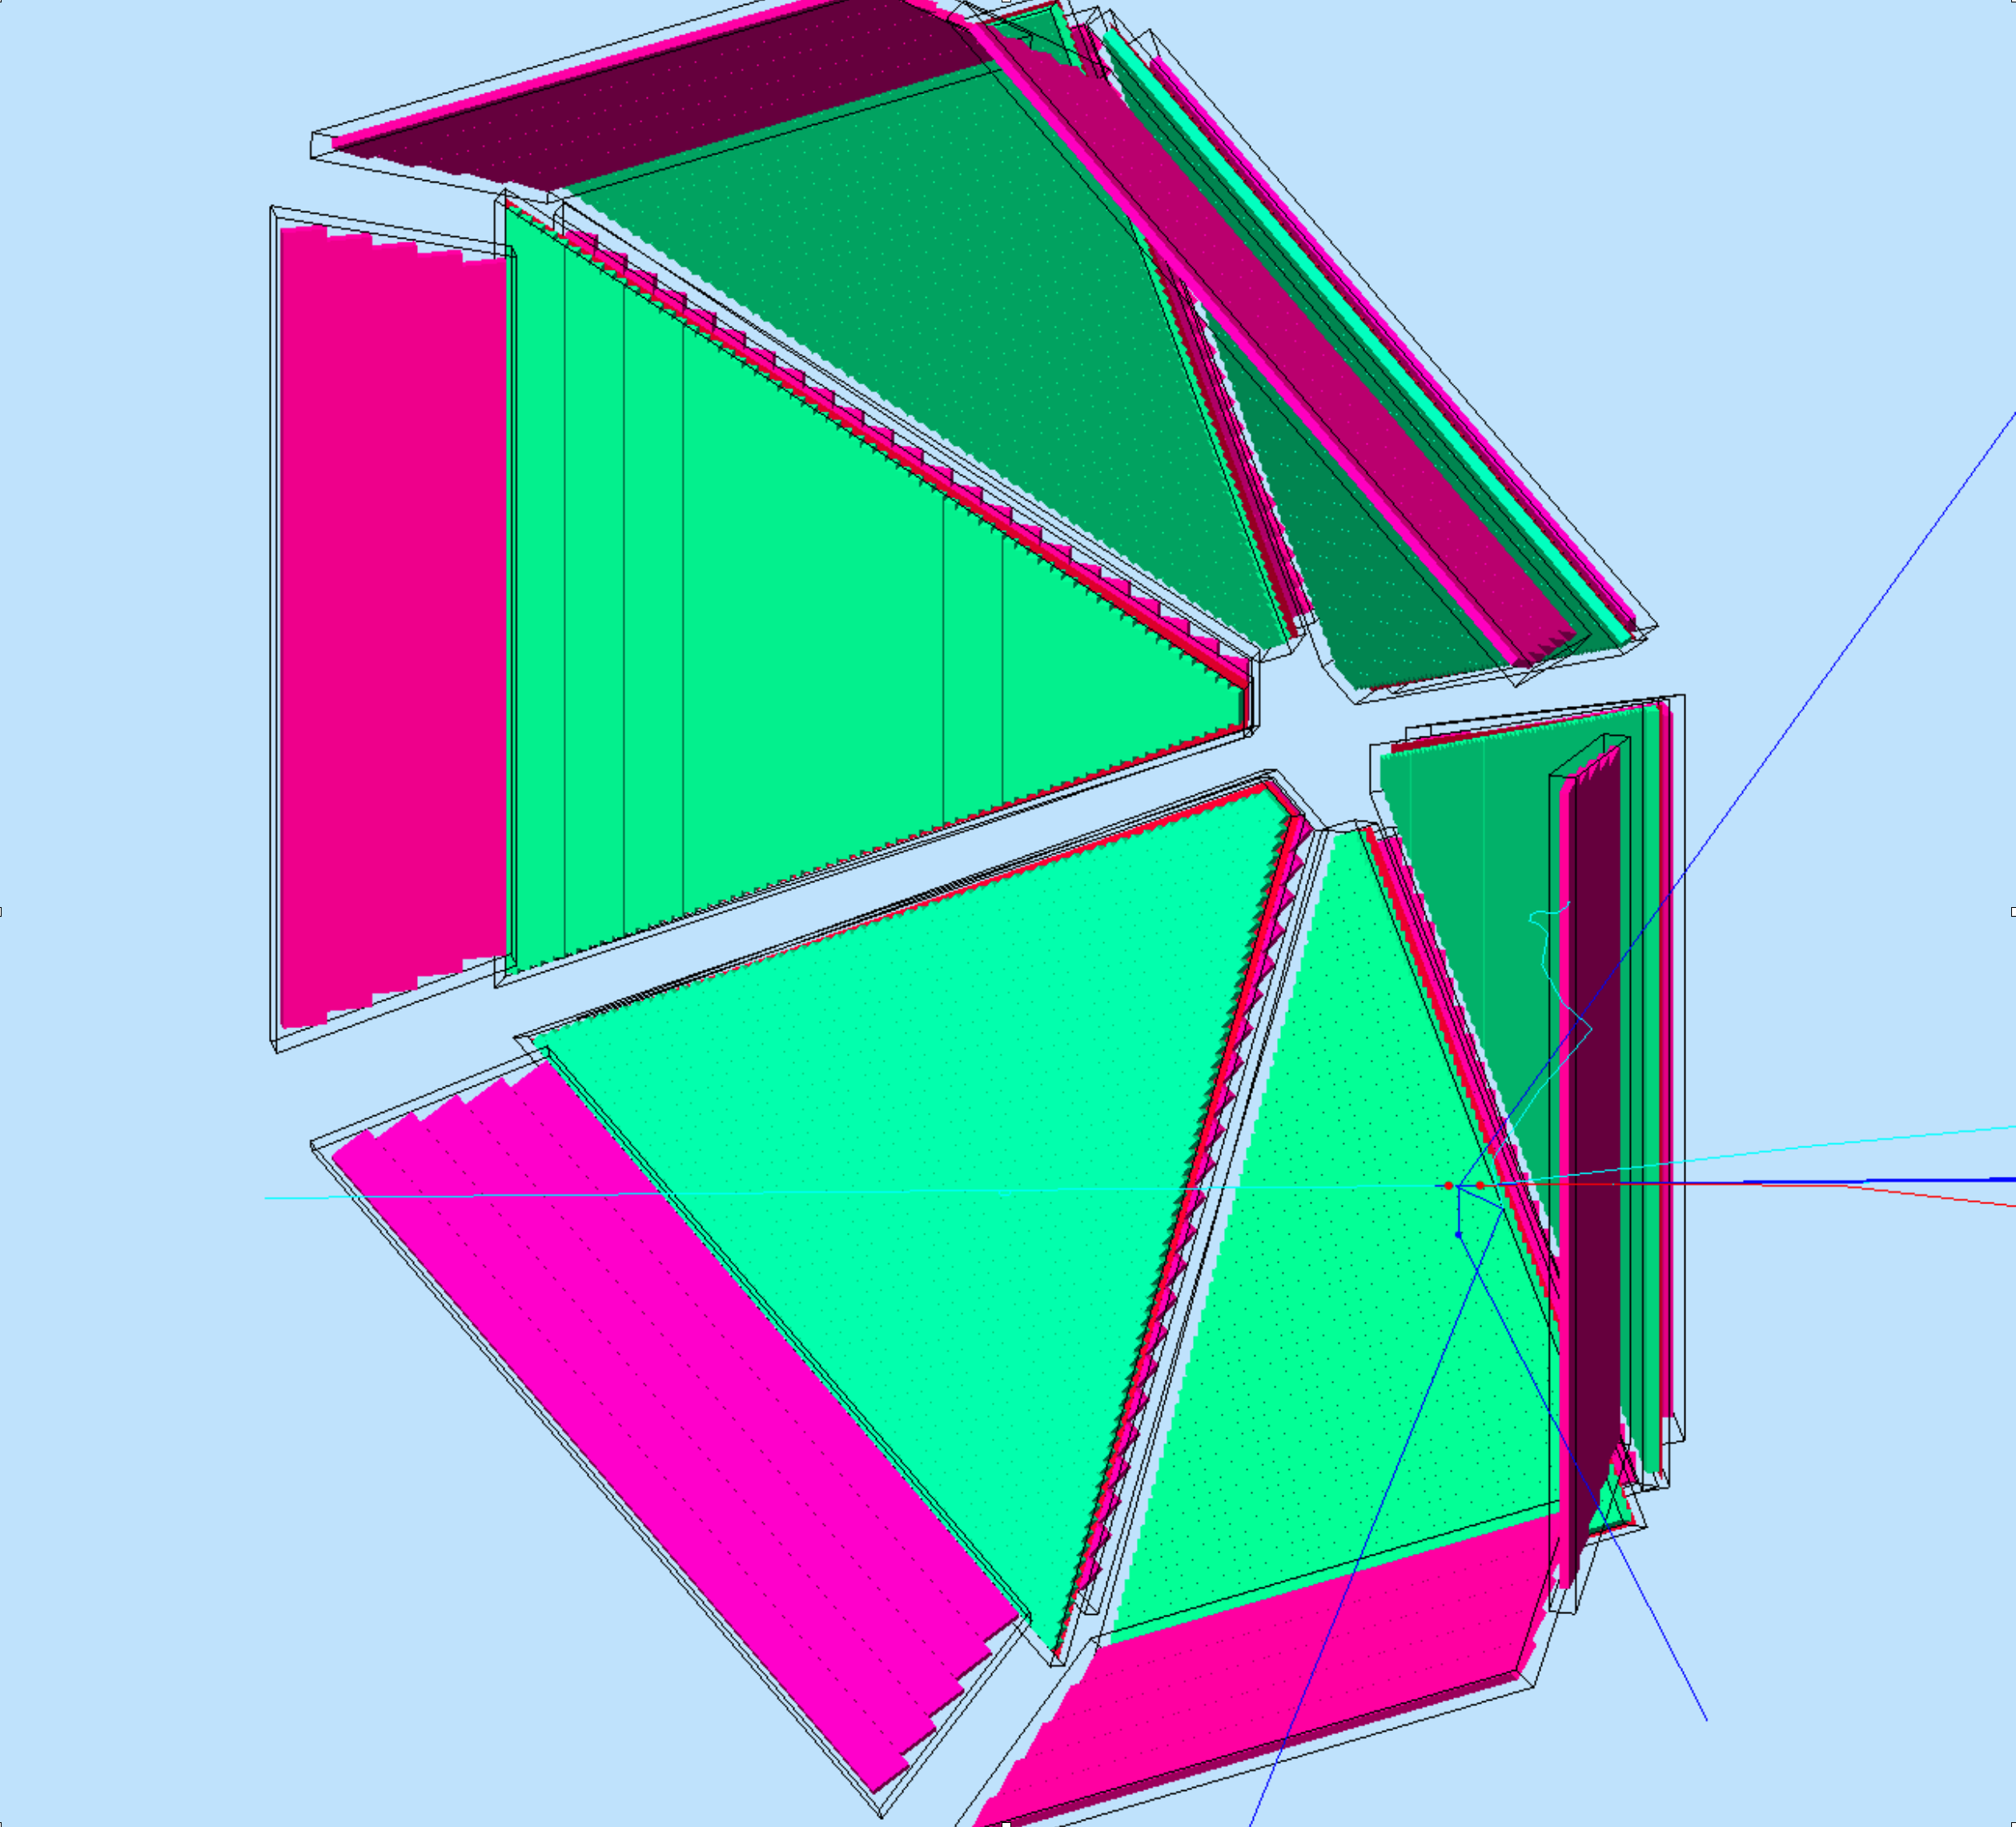
\includegraphics[width=0.99\columnwidth,keepaspectratio]{img/ftofGeometry.png}
	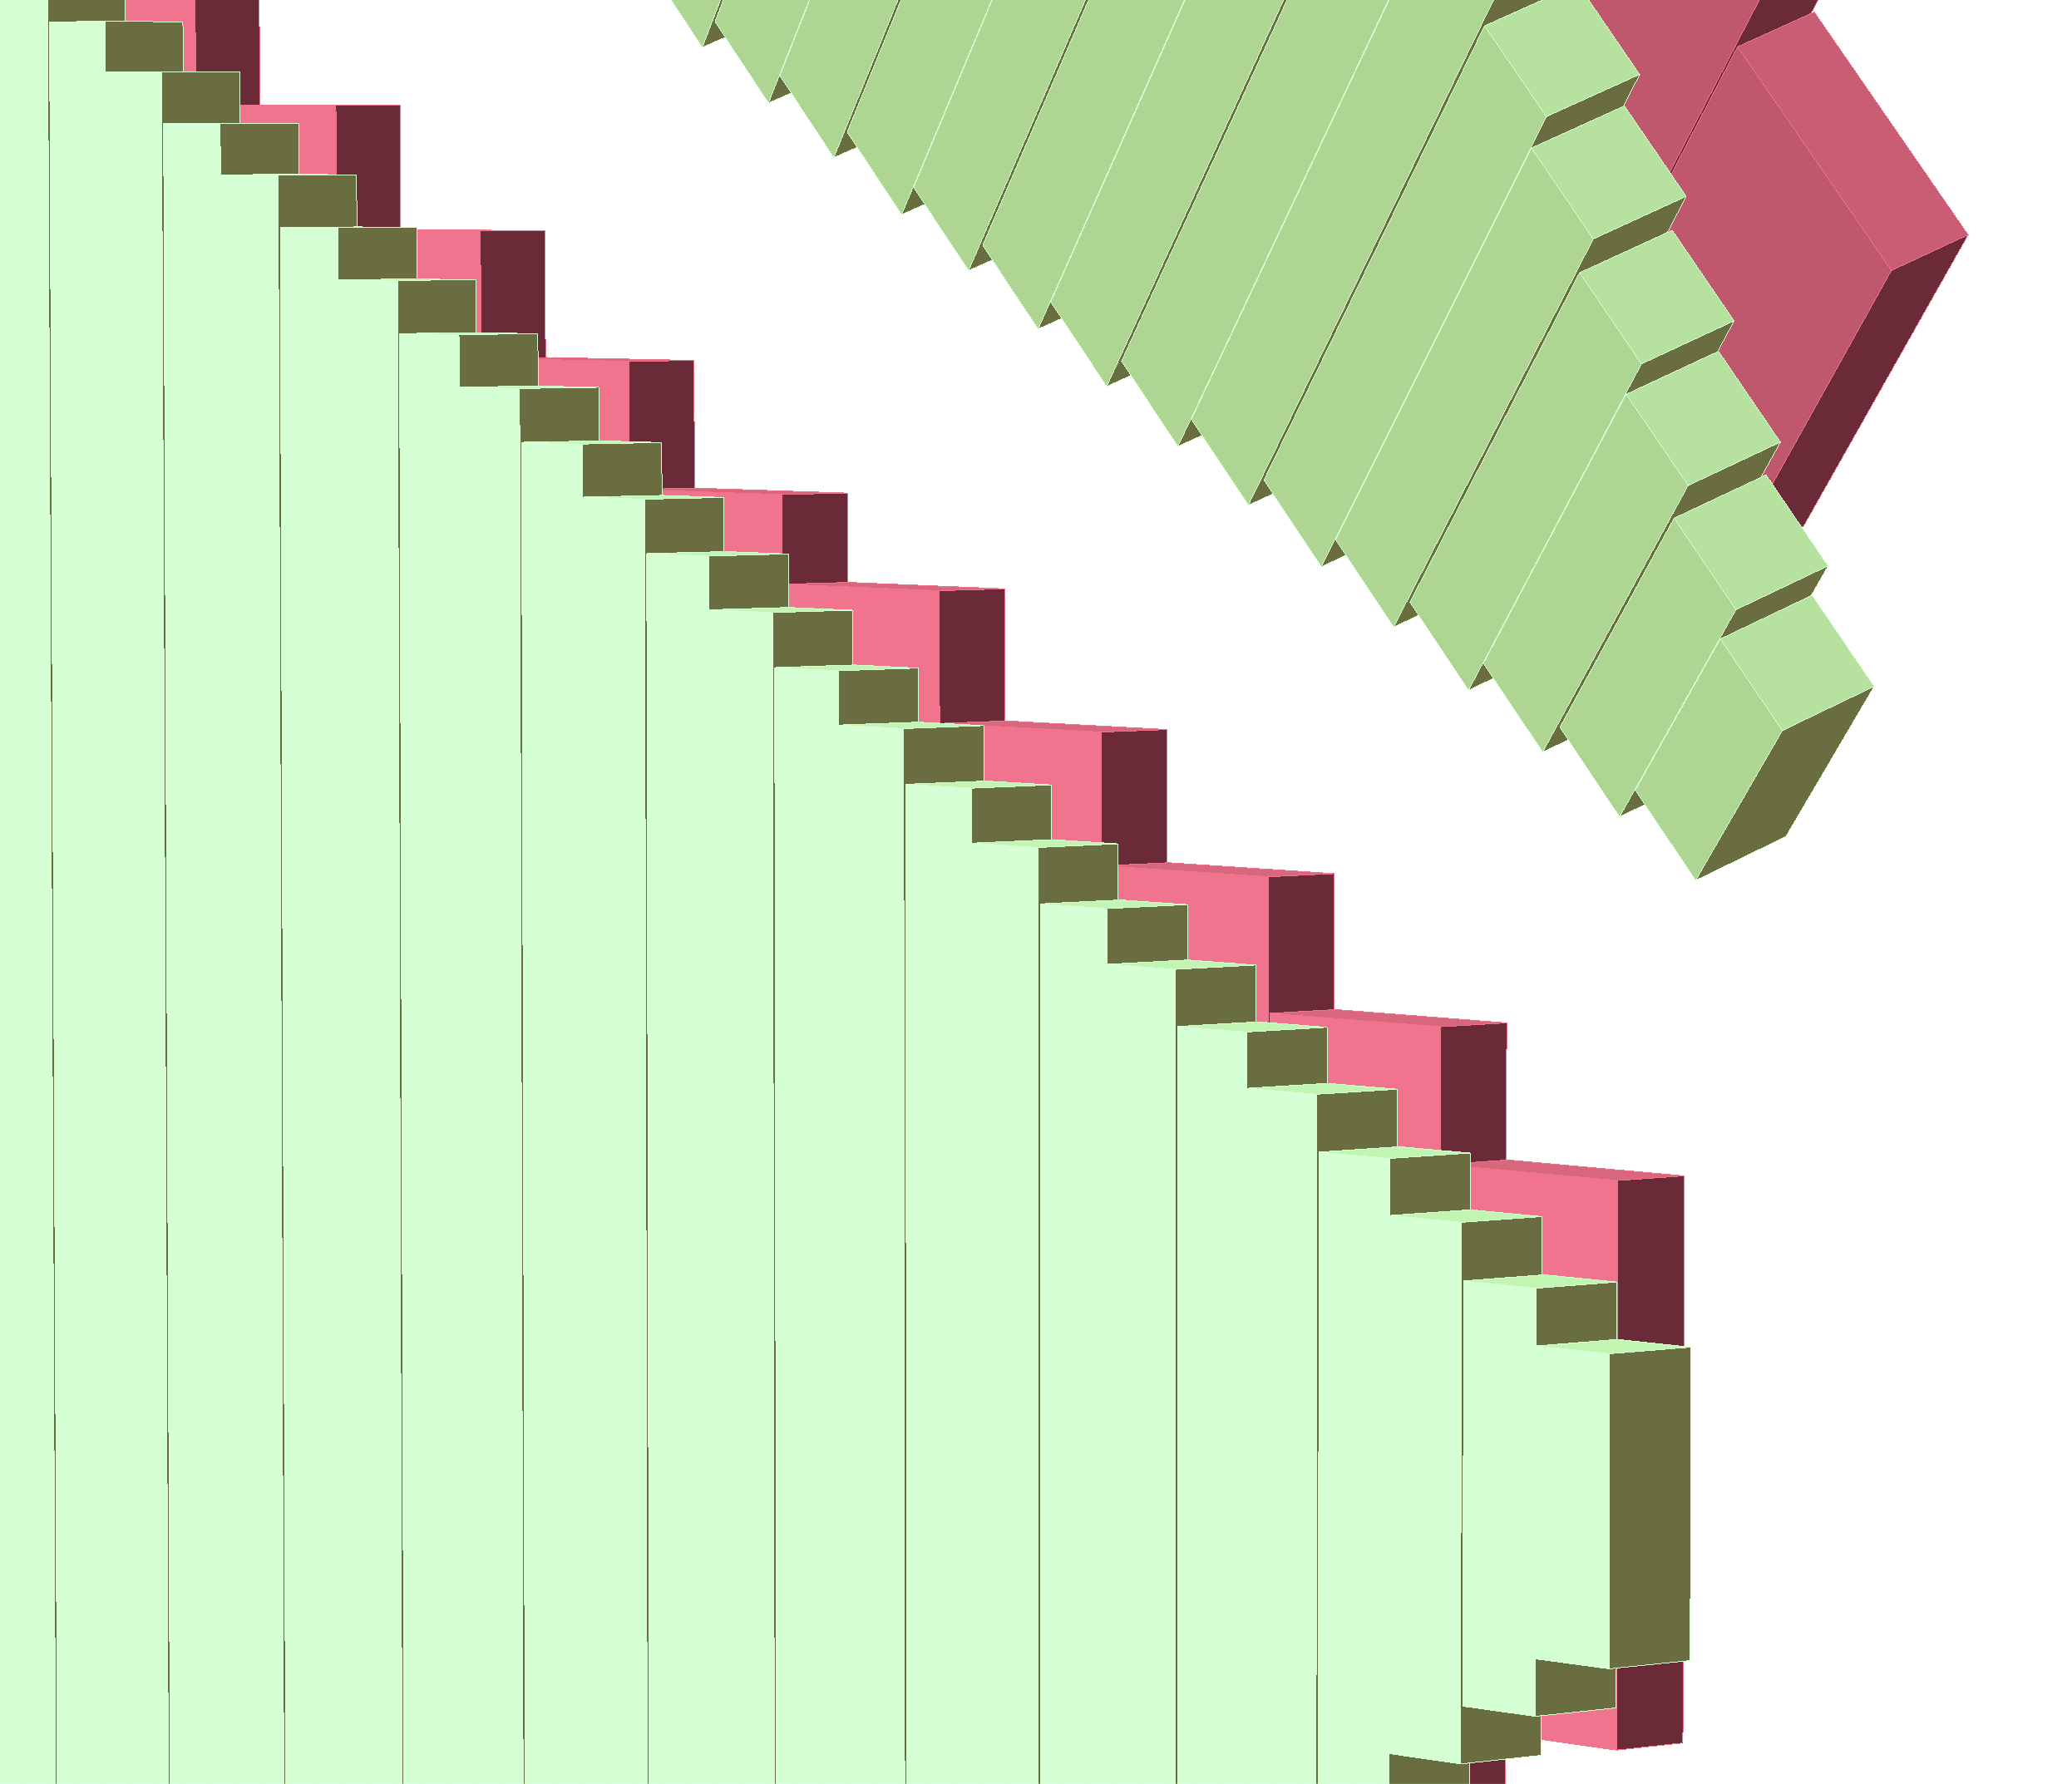
\includegraphics[width=0.99\columnwidth,keepaspectratio]{img/ftofDetail.png}
	\caption{Top: the GEMC implementation of the FTOF geometry. Beam is incident from the left.
             The paddles are G4Boxes embedded in trapezoids
             representing the mother volumes of each panel. A 6 GeV pion is shown, producing one hit (white circle) in each FTOF panel
             in the CLAS12 Forward Detector sector 4.
             Bottom: a zoom-in of the implementation shows the details of the individual paddles for panel-1b (inner,
             in front) and panel-1a (outer). }
	\label{fig:ftofGeometry}
\end{figure}

\subsubsection{Process ID}

Each hit in the paddles produces two hits with the identifier variable ``side'' set to 0
(for the left side PMT) and 1 (for right side PMT).
The hits are then processed independently through the FTOF hit process routine.

\subsubsection{Digitization}

The energy deposited is reduced based on the hit position on the paddle using the calibrated light attenuation length.
It is then corrected by a gain factor to account for the fact that the high voltages (HV) are adjusted so that
the average left/right ADC geometric mean is independent of counter length and hit position.

The corrected energy is converted to the number of photons $N_{th}$ using the constant 500 photons/MeV
which was estimated from data.
A Poissonian is used to calculate the actual number of photons $N_{actual}$ and the resulting ``smeared'' energy
is the converted to ADC using the FADC conversion factor.
An example of the smeared ADC for the right paddles as a function of hit position is shown in \F{ftofAtten}.

\begin{figure}
	\centering
	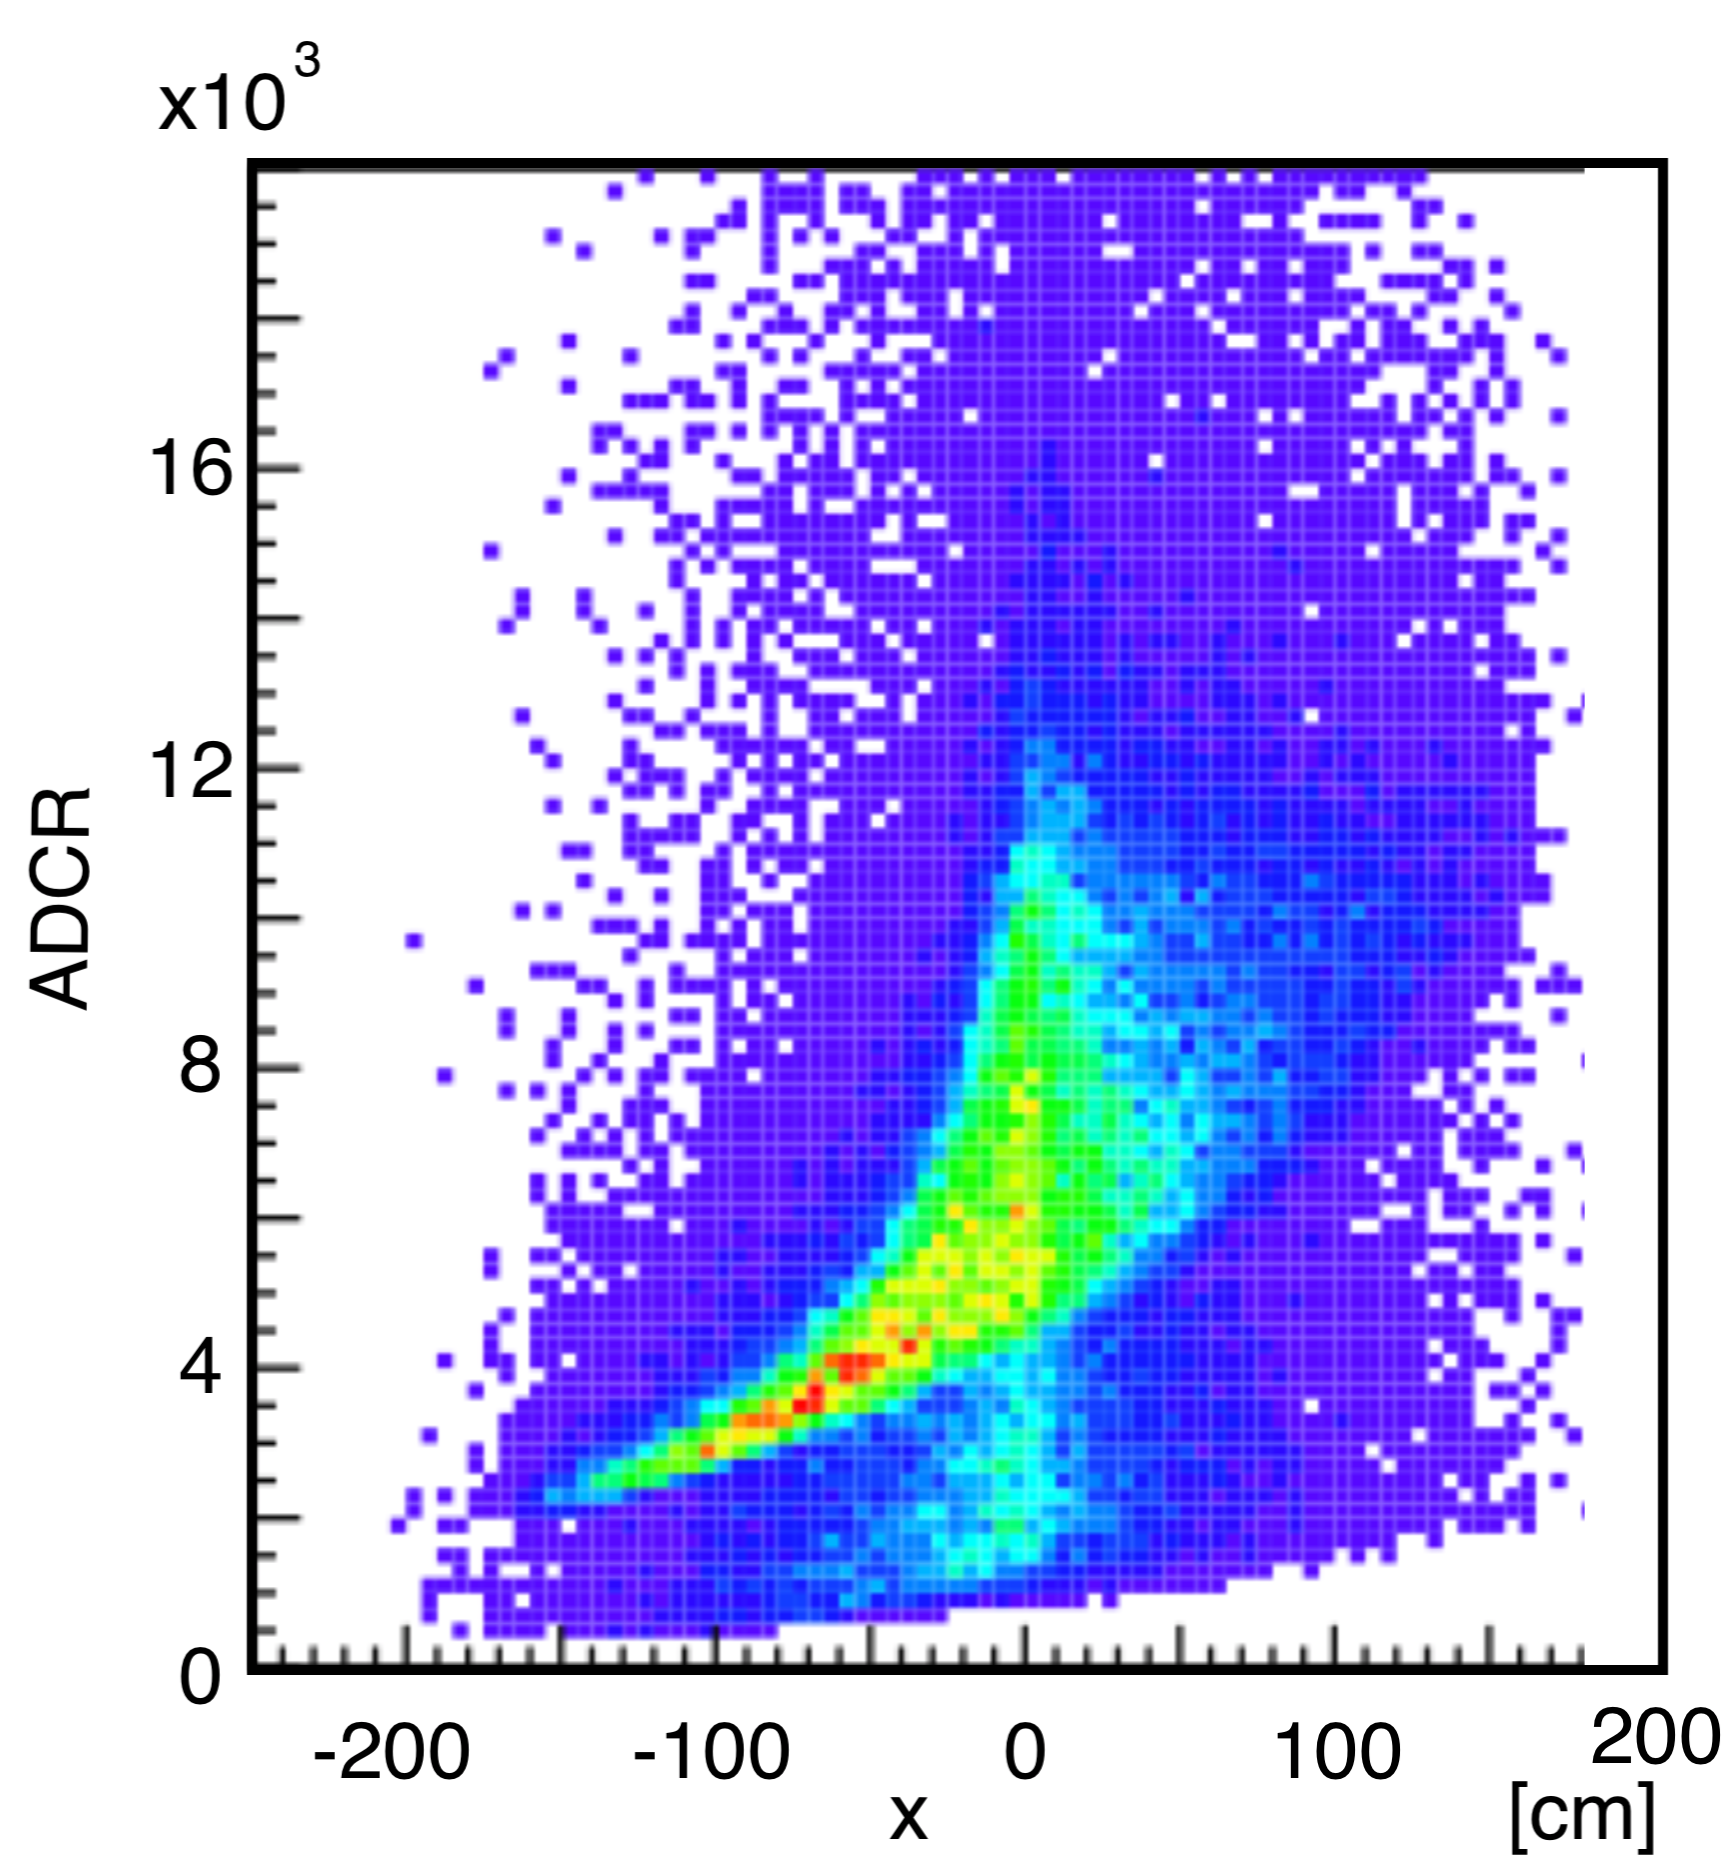
\includegraphics[width=0.99\columnwidth,keepaspectratio]{img/ftofAtten.png}
	\caption{The ADC of the FTOF right paddle PMTs as a function of the relative position of the hit in the paddle.
             The effects of attenuation length and smearing using realistic constants from the CCDB database make
             the FTOF simulation response very similar to the real data.}
	\label{fig:ftofAtten}
\end{figure}

The hit time is processed using:

\begin{itemize}
	\item the effective velocity (from CCDB);
	\item the time-walk correction, calculated from the smeared energy;
	\item a panel to panel timing offset factor (from CCDB);
	\item a left/right time offset factor (from CCDB);
	\item an RF correction (from CCDB).
\end{itemize}

The time is then smeared by a resolution read from CCDB using a Gaussian function and then digitized using a TDC conversion factor.
The digitized output bank variables are summarized in Table \ref{tab:ftofBank}.

\begin{table}[h]
	\begin{center}
		\begin{tabular}{| c | c | c |}
			\hline \hline
			Variable  & Description                                 \\
			\hline
              sector  &                             sector number   \\
               layer  &               layer (1: 1A, 2: 1B, 3: 2)   \\
              paddle  &                             paddle number   \\
                side  &                PMT side (0 Left, 1 Right)   \\
                 ADC  &                                       ADC   \\
                 TDC  &                                       TDC   \\
                ADCu  &                             ADC unsmeared   \\
                TDCu  &                             TDC unsmeared   \\
                hitn  &                                hit number   \\
			\hline \hline
		\end{tabular}
	\end{center}
	\caption{The digitized FTOF bank.}\label{tab:ftofBank}
\end{table}


The time window  of the FTOF is set to 400 ns: all Geant4 steps within the same paddle and time window are collected in one hit.


